%\textcolor{red}{\hrulefill \textsc{Unfinished Section}\hrulefill}  \\
An alternative solution is obtained by simply postulating that the MSSM should be extended by a gauged $U(1)_{B-L}$ symmetry (of which \emph{R}-parity is a discrete subgroup) which is spontaneously broken at some scale.
This breaks $L$ and, hence, \BL symmetry.
However, $B$ remains unbroken and therefore proton decay continues to be suppressed below its present experimental bounds.
However, the parameters of the \BL MSSM must still be chosen so as to adequately suppress lepton number violating processes.
This reproduces the exact MSSM particle spectrum with an additional three right handed neutrino chiral multiplets as well as a $Z'_{B-L}$ (and its superpartner) from the broken symmetry.
Below the scale of both spontaneous \BL and SUSY breaking, the observable sector of this theory contains precisely the particle spectrum and gauge group of the Standard Model.
This is known as the \BL Minimal Supersymmetric Standard Model as described from the ``bottom-up'' approach.
Also note that a ``top-down'' approach was shown to be possible in a series of papers \cite{Ambroso:2009sc,Ambroso:2010pe,Braun:2005nv,Ovrut:2014rba,Ovrut:2012wg,Ovrut:2015uea,Ambroso:2009jd} where this exact \BL MSSM is recovered as the low energy theory of heterotic superstring/M-theory.
The continuous $U(1)_{B-L}$ symmetry arising naturally as a consequence of the compactification of heterotic M-theory, which has long been known in a non-supersymmetric context to be the minimal extra gauging of the standard model that remains quantum mechanically anomaly free~\cite{Dumitru:2018jyb}.
That is, the gauged $U(1)_{B-L}$ that arises in this context gives a ``natural way'' to suppress unwanted baryon and lepton number violating decays.
For all of these reasons, \emph{the \BL MSSM appears to be the simplest possible phenomenologically realistic theory of heterotic superstring/M-theory; being exactly the MSSM with right-handed
neutrino chiral supermultiplets and spontaneously broken R-parity}~\cite{Dumitru:2018nct}
The post-EWKSB particle content of the \BL MSSM is illustrated in Figure~\ref{fig:theory:particlesSUSYBL}. 
\begin{figure}[htb]
  \begin{center}
    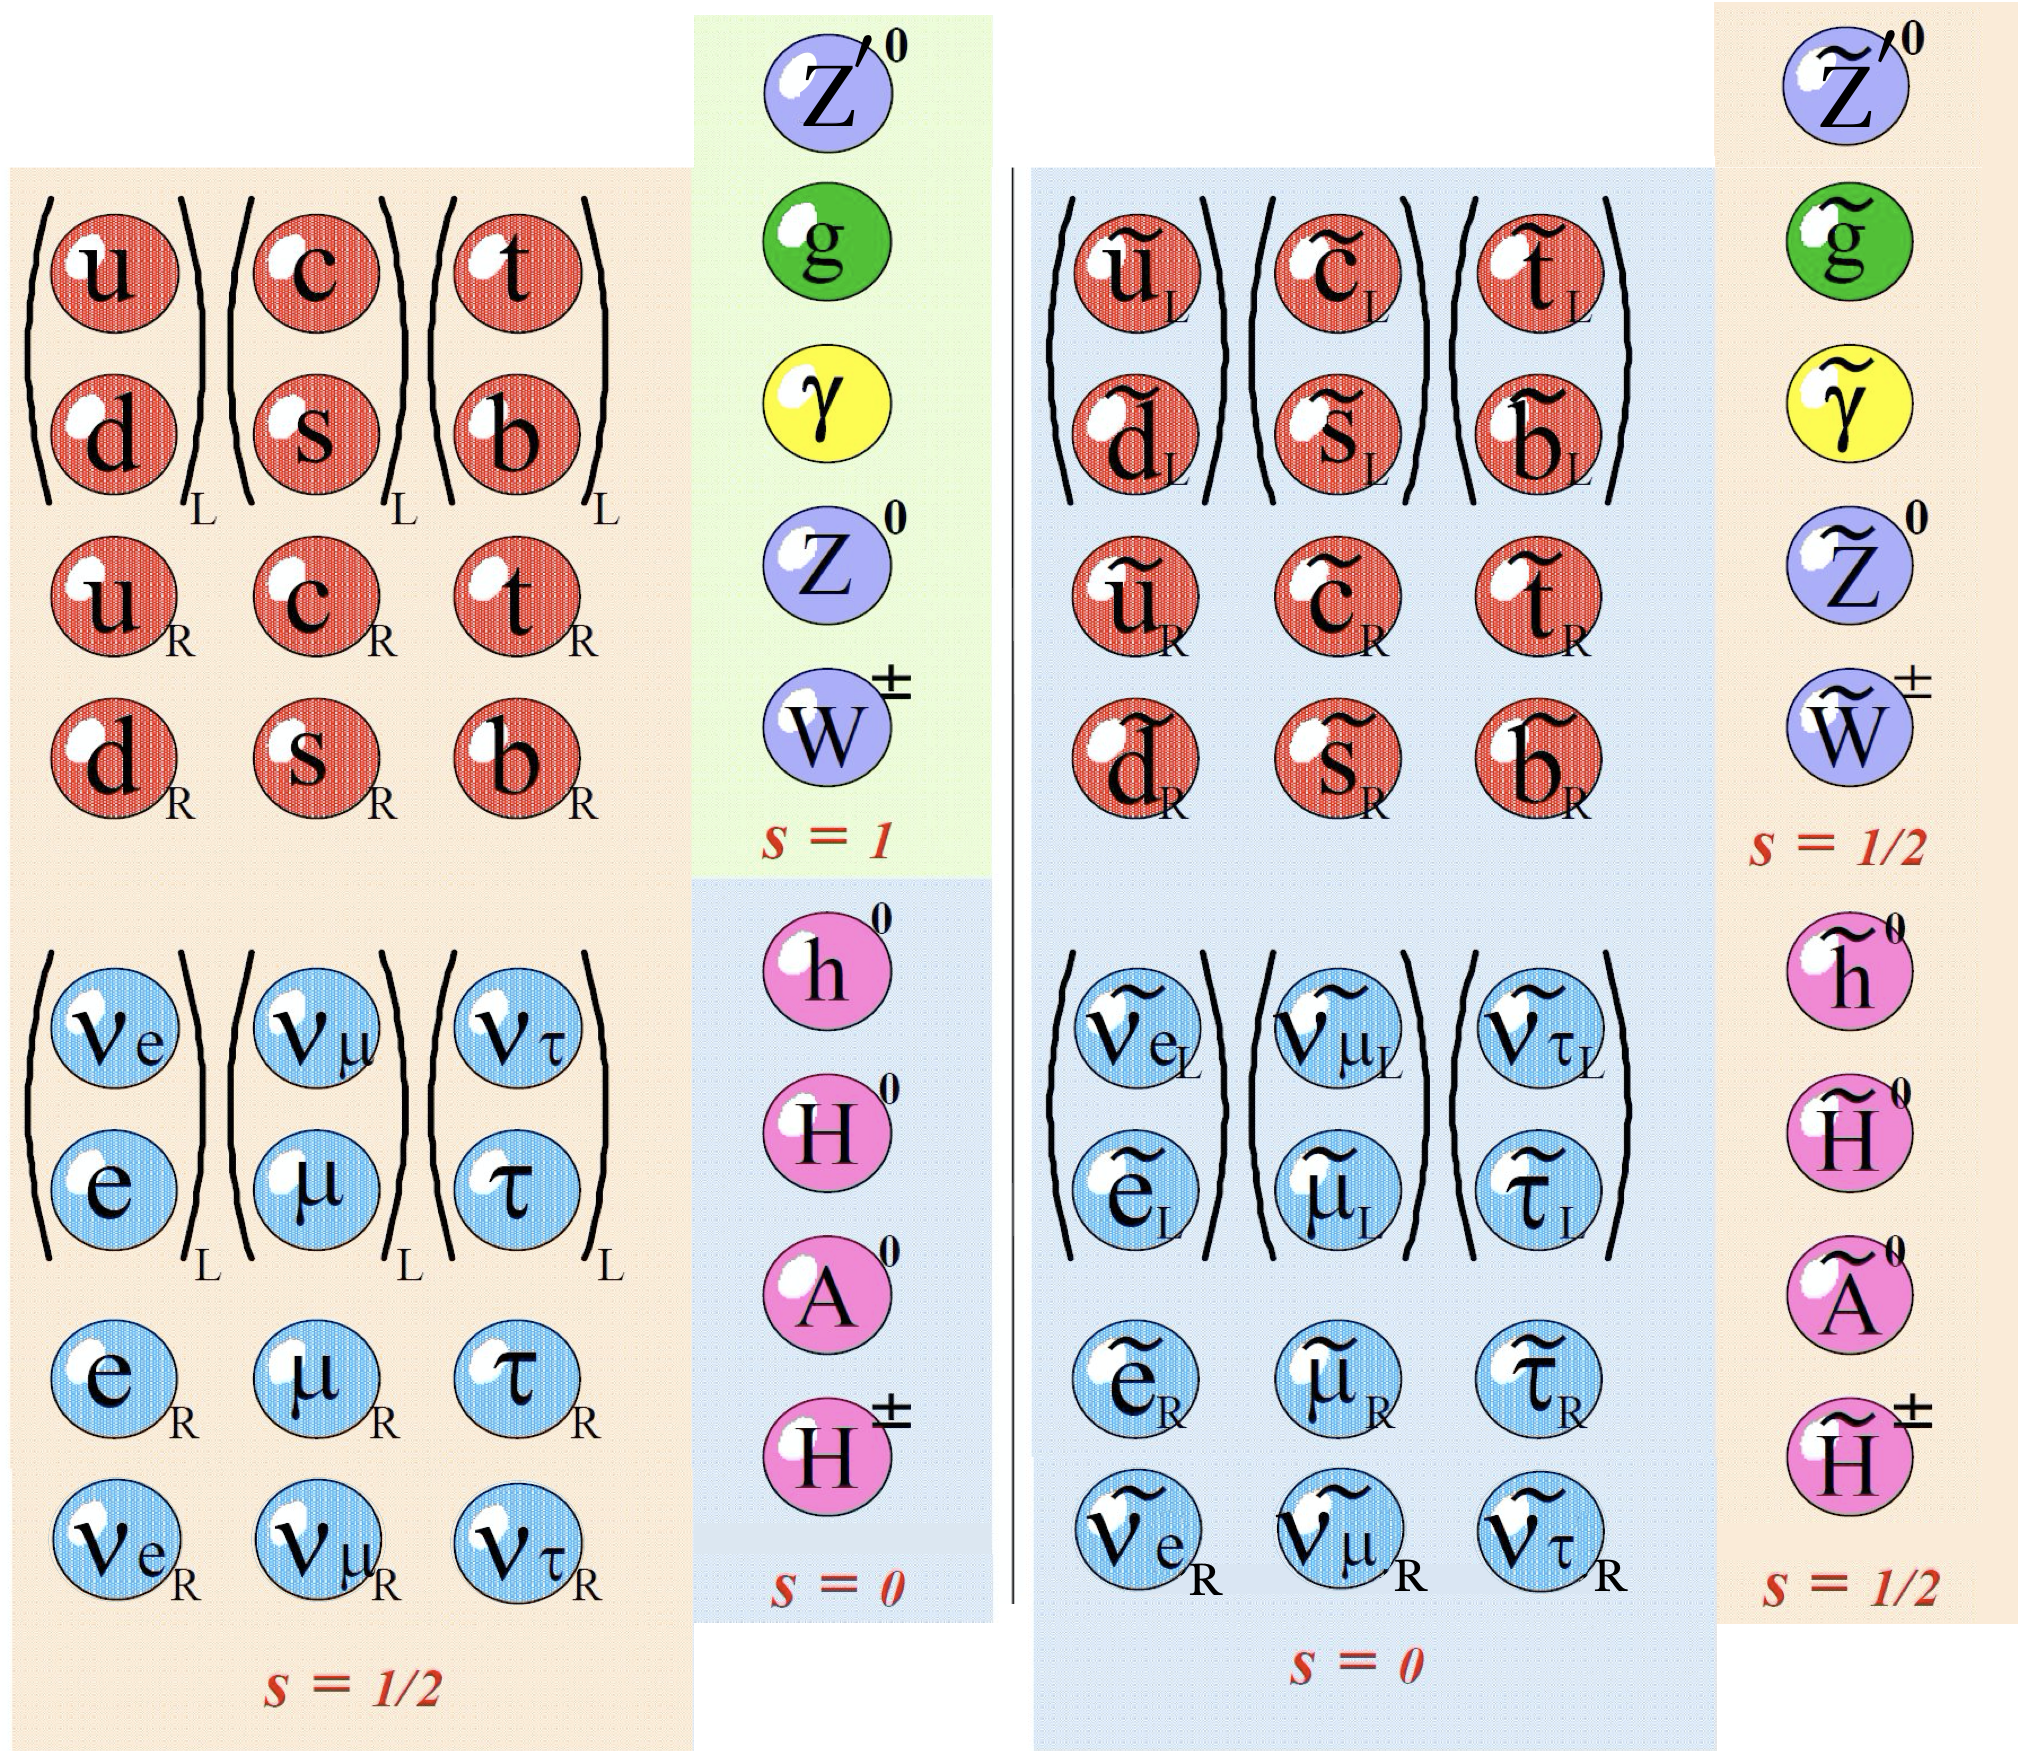
\includegraphics[width=0.98\textwidth]{figs/theory/SMtoBLSUSYparticleContent.png}
  \end{center}
  \caption[Minimal SUSY \BL Model particle content]{The post-EWKSB particle content of the \BL MSSM.
  Referring back to Figure~\ref{fig:theory:particlesSUSY} we note the addition of both right-handed neutrinos and sneutrinos. 
  A $Z'$ and its superpartner coming from the broken $U(1)_{B-L}$ symmetry are also added~\cite{KEK:2021}}
  \label{fig:theory:particlesSUSYBL}
\end{figure}
The gauge group for the \BL MSSM is then
\begin{equation}
    SU(3)_{C} \times SU(2)_{L} \times U(1)_{Y} \times U(1)_{B-L}
\end{equation}
However, as discussed in detail in~\cite{Ovrut:2012wg}, it is equivalent and convenient to choose the gauge group to be
\begin{equation}
    SU(3)_{C} \times SU(2)_{L} \times U(1)_{3R} \times U(1)_{B-L}
\end{equation}
where $U(1)_{3R}$ is the canonical Abelian subgroup of $SU(2)_{R}$.
It was shown in~\cite{Ovrut:2012wg} that there is no kinetic mixing between the field strengths of $U(1)_{3R}$ and $U(1)_{B-L}$ at any momentum scale, and that this is the unique basis with this property.
This vastly simplifies the solution of the RGEs and therefore the analyses done in the cited works work in this gauge group and so as to remain consistent the literature we will as well.
The particle content corresponding to this gauge group is illustrated in Figure~\ref{fig:theory:particlesSUSYBLpreB-LSB}.
\begin{figure}[tb]
  \begin{center}
    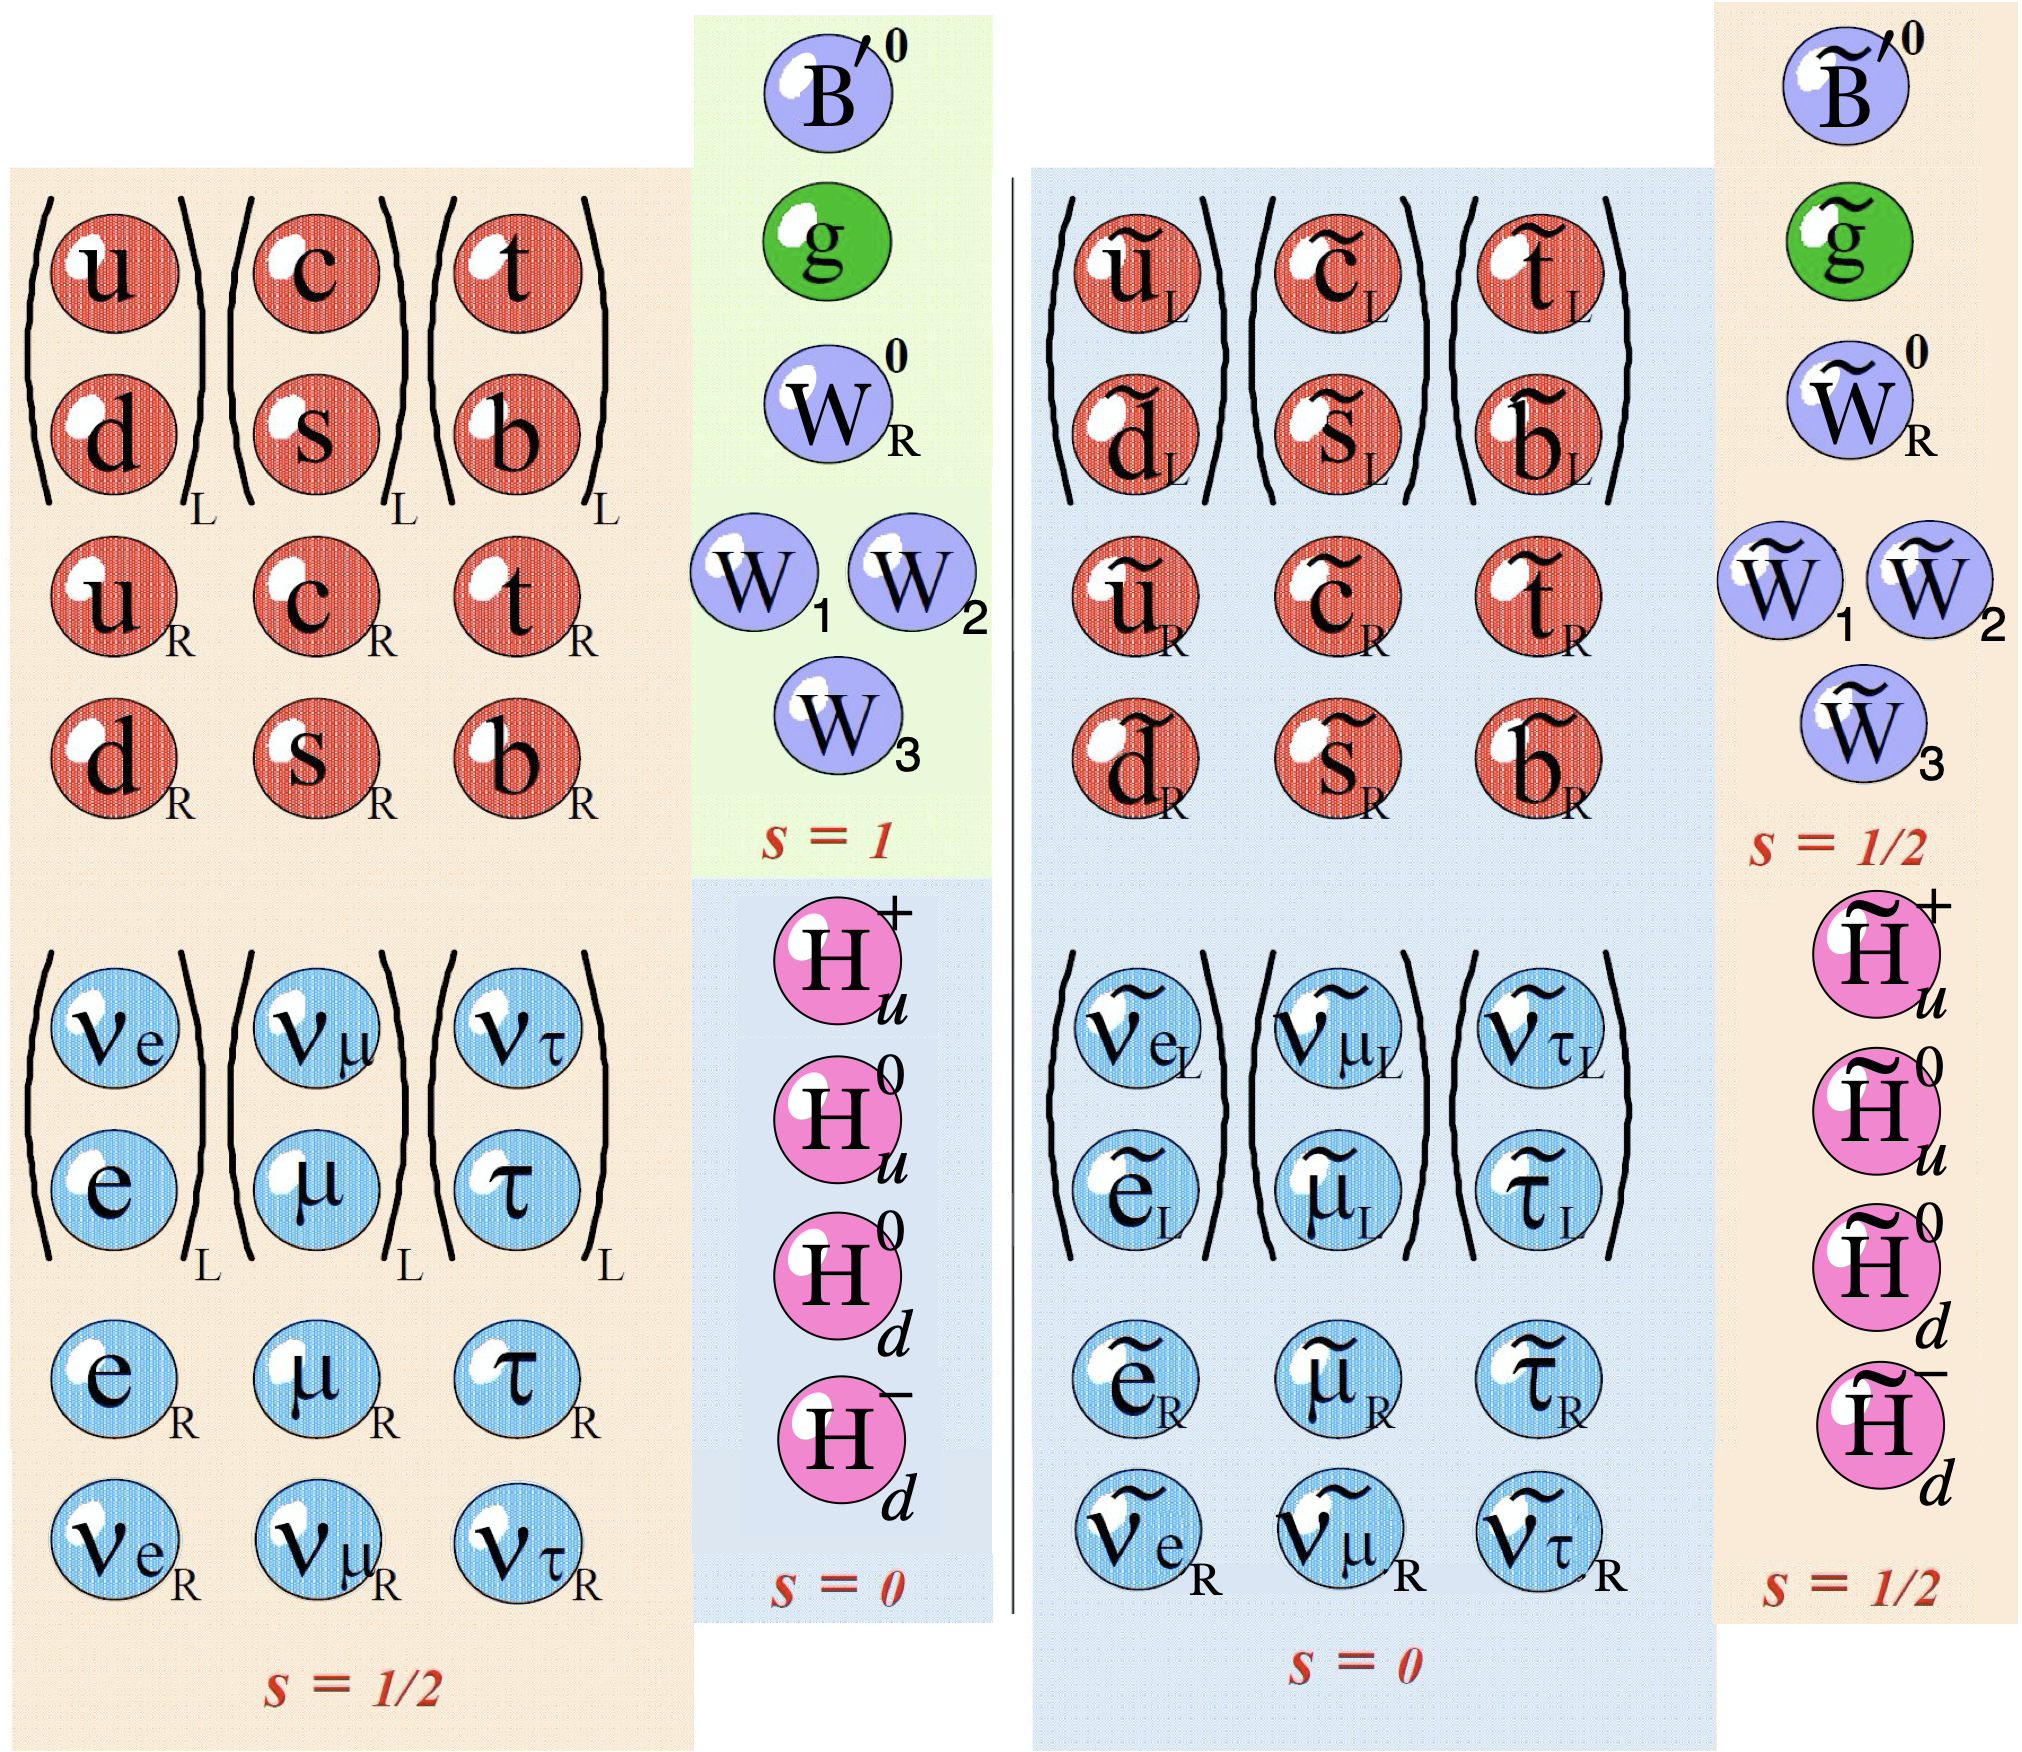
\includegraphics[width=0.98\textwidth]{figs/theory/ParticlesRPVSUSYpreB-LSB.png}
  \end{center}
  \caption[Minimal SUSY \BL Model particle content, pre-\BL breaking]{\cite{KEK:2021}}
  \label{fig:theory:particlesSUSYBLpreB-LSB}
\end{figure}
Note the Blino ($B'^{0}$) and Rhino ($W_{R}^{0}$), corresponding to $U(1)_{B-L}$ and $U(1)_{3R}$ gauge symmetries respectively, in the Figure. 

\subsection{Phenomenology of a Broken $B-L$ Symmetry}
In this theory the $U(1)_{B-L}$ symmetry can in principle be spontaneously broken by the right-handed sneutrino acquiring an non-vanishing vacuum expectation value (VEV).
It was proven that this VEV could dynamically occur via radiative breaking in the \BL MSSM using a full renormalization group (RG) analysis in~\cite{Ambroso:2009jd}.
Of course, the symmetry must be spontaneously broken at a scale sufficiently high to account for the fact that its associated massive vector boson $Z'_{B-L}$ has, so far, not been observed.

A consequence of the breaking of $U(1)_{B-L}$ is the introduction of \emph{R}-Parity violating terms, which will not significantly affect the mass eigenstates, \emph{but do introduce mixing between the gauginos and the standard model charged leptons}~\cite{Dumitru:2018jyb}.
These mixings are central to this thesis as these are what allow for RPV decays and result in interesting signatures not well covered by standard SUSY searches at collider experiments.
%is that the superpartners of the charged Higgs, charged \Wboson bosons, and SM charged leptons now mix.
Continuing to work in the $SU(3)_{C} \times SU(2)_{L} \times U(1)_{3R} \times U(1)_{B-L}$ basis, the charged\footnote{electromagnetically} mixed mass eigenstates, called \emph{charginos}, are related to the gauge eigenstates by unitary matrices $\mathcal{V}$ and $\mathcal{U}$ defined by 
%We also note that making N = 1 (MSSM) SUSY a local symmetry produces gravitation as the associated gauge field, although in the form of a gravity supermultiplet containing the gravitino as well as the graviton~\cite{Dumitru:2018jyb}.
%That is, the existence of N = 1 supersymmetry puts gravity on par with the strong, weak and electromagnetic gauge interactions~\cite{Dumitru:2018jyb}.
\begin{align}
    \begin{pmatrix}
       \tilde\chi_{1}^{-} \\
       \tilde\chi_{2}^{-} \\
       \tilde\chi_{3}^{-} \\
       \tilde\chi_{4}^{-} \\
       \tilde\chi_{5}^{-} 
    \end{pmatrix}
    =\mathcal{U} 
    \begin{pmatrix}
      \tilde W^{-}\\ 
      \tilde H_{d}^{-}\\ 
      e^{-} \\ 
      \mu^{-} \\ 
      \tau^{-} 
    \end{pmatrix},\hspace{1.0cm}
    \begin{pmatrix}
       \tilde\chi_{1}^{+} \\
       \tilde\chi_{2}^{+} \\
       \tilde\chi_{3}^{+} \\
       \tilde\chi_{4}^{+} \\
       \tilde\chi_{5}^{+} 
    \end{pmatrix}
    =\mathcal{V} 
    \begin{pmatrix}
      \tilde W^{+} \\ 
      \tilde H_{u}^{+} \\ 
      e^{+} \\ 
      \mu^{+} \\ 
      \tau^{+} 
    \end{pmatrix}
\end{align}
Where the explicit values for the entries in  $\mathcal{V}$ and $\mathcal{U}$ can be found in~\cite{Dumitru:2018jyb}.
For the analogous neutral mass eigenstates, \emph{neutralinos}, we have an even more complicated situation.
First, it has been shown that mixing with the first- and second-family right-handed neutrino would lead to active sterile neutrino oscillations~\cite{Dumitru:2018jyb}.
Unless and until there is more experimental evidence of such oscillations, we will assume that they do not exist. 
Therefore, the mixing with the first and second-family right-handed neutrinos is negligible and we include only mixing with the three families of left-handed neutrinos and the third-family right-handed neutrino~\cite{Dumitru:2018jyb}.
The neutralinos are then related to the gauge eigenstates by unitary matrix $\mathcal{N}$ defined by
\begin{align}
    \begin{pmatrix}
       \tilde\chi_{1}^{0} \\
       \tilde\chi_{2}^{0} \\
       \tilde\chi_{3}^{0} \\
       \tilde\chi_{4}^{0} \\
       \tilde\chi_{5}^{0} \\
       \tilde\chi_{5}^{0} \\
       \tilde\chi_{5}^{0} \\
       \tilde\chi_{5}^{0} \\
       \tilde\chi_{5}^{0} 
    \end{pmatrix}
    =\mathcal{N} 
    \begin{pmatrix}
      \tilde W_{R}\\ 
      \tilde W^{0}\\ 
      \tilde H_{d}^{0}\\ 
      \tilde H_{u}^{0}\\ 
      \tilde B'\\ 
      \nu_{3}^{c}\\
      \nu_{e}\\
      \nu_{\mu}\\
      \nu_{\tau}
    \end{pmatrix}
\end{align}
Where again the explicit values for the entries in  $\mathcal{N}$ can be found in~\cite{Dumitru:2018jyb}.
Now due to the relative smallness of the RPV couplings we expect RPV decays primarily coming from the LSP of the theory, as heavier charginos/neutralinos would prefer RPC decay channels.
So it then becomes important to determine if the \chono\footnote{The lightest chargino and neutralino state respectively} are even likely candidates to be the LSP in the \BL MSSM. 
An extensive study involving the statistical scanning over all dimensionful parameters of the soft SUSY breaking terms was done in \cite{Dumitru:2018jyb} and does motivate \chono  as likely LSPs in the \BL MSSM.
This scan is discussed in more detail in Chapter~\ref{ch:rpvthreel} where additional experimental considerations are taken into account as well.


%\begin{figure}[htb]
%  \begin{center}
%    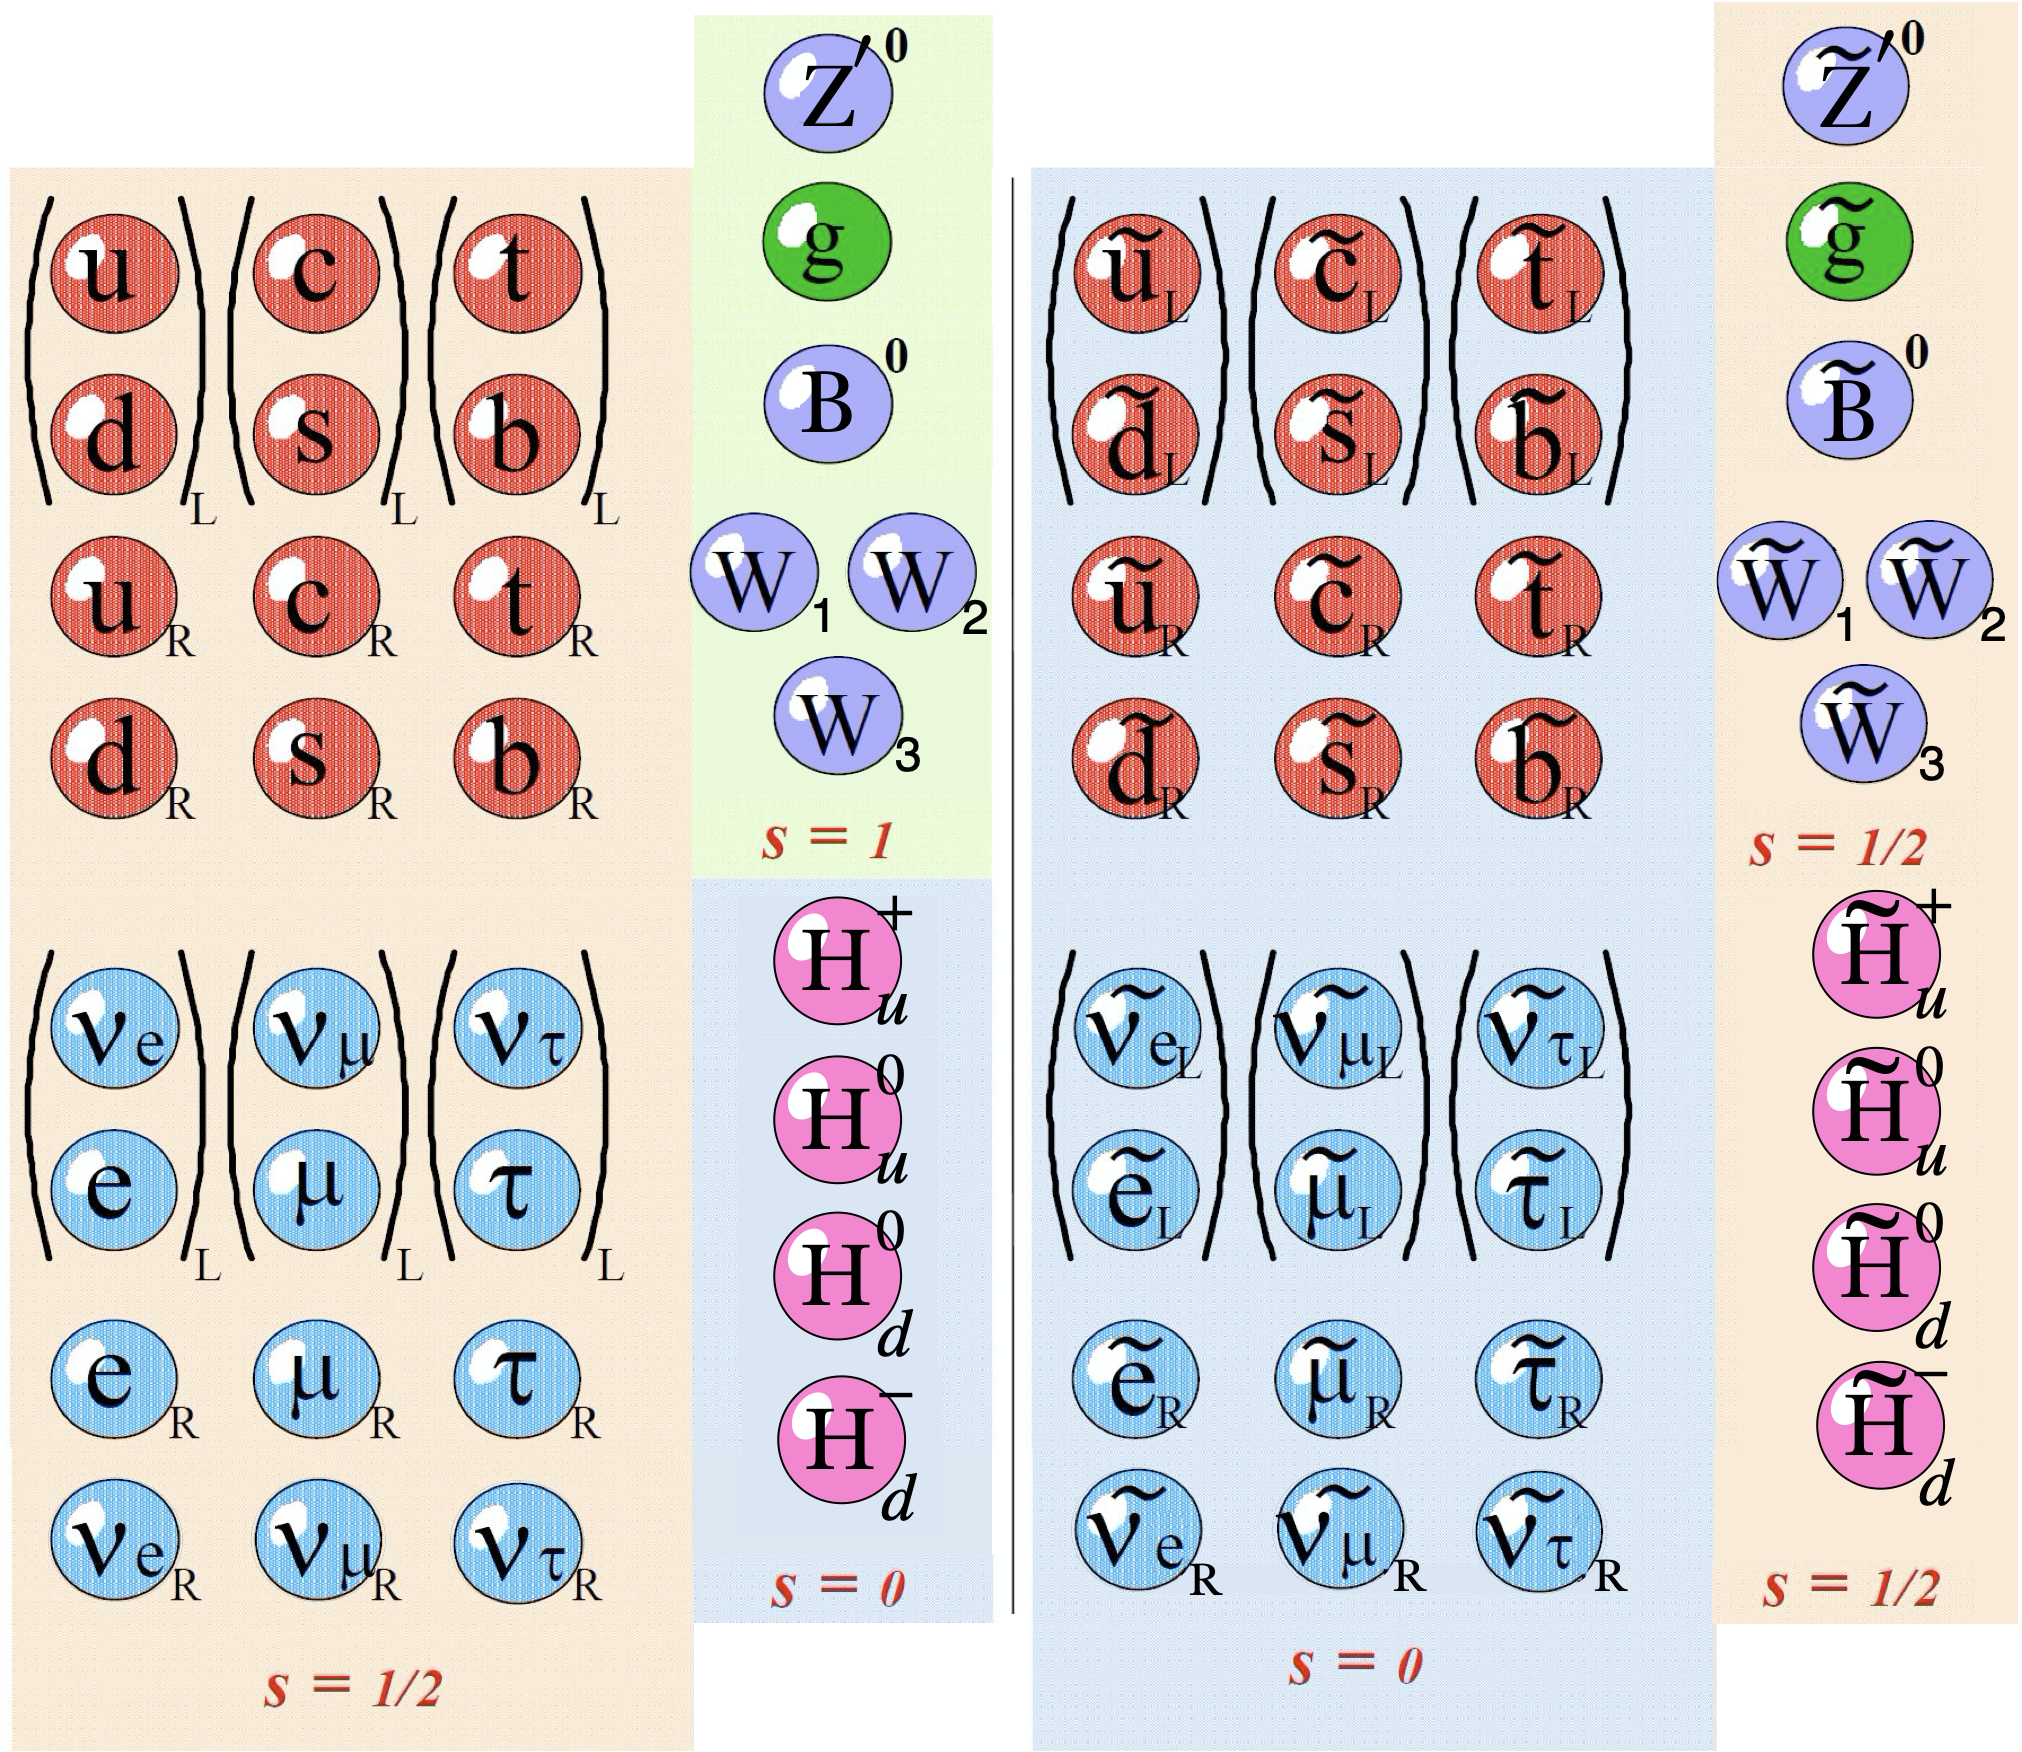
\includegraphics[width=0.98\textwidth]{figs/theory/ParticlesRPVSUSYpreEWKSB.png}
%  \end{center}
%  \caption[Minimal SUSY \BL Model particle content, pre-EWKSM]{\cite{KEK:2021}}
%  \label{fig:theory:particlesSUSYBLpreEWKSB}
%\end{figure}

%It is important to note that despite the violation of \emph{R}-parity, an LSP gravitino can live long enough to potentially play the role of dark matter~\cite{Buchmuller:2007ui,Takayama:2000uz}.